\documentclass[12pt]{article}

\usepackage[utf8]{inputenc}
\usepackage[T1]{fontenc}
\usepackage[polish,provide=*]{babel}
\usepackage{lmodern}
\usepackage{amsmath}
\usepackage{latexsym,amsfonts,amssymb,amsthm,amsmath}
\usepackage{enumitem}
\usepackage{hyperref}
\usepackage{float}
\usepackage{graphicx}
\usepackage{subcaption}
\usepackage{booktabs}
\graphicspath{{./images/}}

\setlength{\parindent}{0in}
\setlength{\oddsidemargin}{0in}
\setlength{\textwidth}{6.5in}
\setlength{\textheight}{8.8in}
\setlength{\topmargin}{0in}
\setlength{\headheight}{18pt}

\title{Wahadła sprzężone}
\author{Kacper Kłos}

\begin{document}

\maketitle

W poniższym raporcie wyznaczyliśmy współczynnik sprężystości sprężyny trzema metodami. Najpierw zawiesiliśmy sprężynę i podczepialiśmy pod nią ciężarki, mierząc rozciągnięcie. Do punktów pomiarowych dopasowaliśmy zależność liniową, z której parametrów otrzymaliśmy stałą sprężystości \(k_0 = (29{,}34 \pm 0{,}21)\, \mathrm{N\,m^{-1}}\).

Następnie dwa identyczne wahadła połączyliśmy sprężyną na tej samej wysokości i mierzyliśmy osobno drgania w fazie i w przeciwfazie. W oby przypadkach do wyznaczenia częstotliwości wykorzystaliśmy transformację Fouriera. Doświadczenie powtórzyliśmy dla trzech różnych odległości sprężyny od osi obrotu. Dla tych pomiarów średnia ważona stałej sprężystości wyniosła \(k_p = (32{,}4 \pm 2{,}0)\, \mathrm{N\,m^{-1}}\).

Na końcu zbadaliśmy dudnienia obu połączonych wahadeł, wyznaczając stałą sprężystości z dwóch częstotliwości, z jakimi wahadła drgały. Średnia z pomiarów dla trzech odległości sprężyny od osi obrotu wynosi \(k_d = (29{,}6 \pm 2{,}0)\, \mathrm{N\,m^{-1}}\).

\newpage
\section{Wyniki pomiarów}

W raporcie będziemy korzystać ze stałej grawitacyjnej \(g = 9{,}81\, \mathrm{m\,s^{-2}}\).

\subsection{Pomiar statyczny}
Pomiar rozpoczynamy od zawieszenia sprężyny i kolejnego podwieszania ciężarków na jej końcu.
\begin{table}[H]
	\centering
	\begin{tabular}{c|cc}
		\toprule
		\textbf{Nr} & Masa \(m\) [g] & Długość sprężyny \(L\) [cm] \\
		\midrule
		1           & 49{,}14        & 31{,}4                      \\
		2           & 91{,}27        & 32{,}8                      \\
		3           & 151{,}85       & 34{,}8                      \\
		4           & 201{,}43       & 36{,}6                      \\
		5           & 250{,}71       & 38{,}2                      \\
		6           & 299{,}12       & 39{,}7                      \\
		7           & 348{,}18       & 41{,}4                      \\
		\bottomrule
	\end{tabular}
	\caption{Długość sprężyny \(L\) w zależności od masy obciążenia \(m\).}
	\label{tab:spring_mass}
\end{table}

Za błąd pomiarowy długości przyjmujemy \(0{,}3\,\mathrm{cm}\), natomiast błąd wagi na poziomie \(0{,}01\,\mathrm{g}\) uznajemy za pomijalnie mały w porównaniu z błędem długości.

Do zebranych danych dopasowujemy równanie liniowe
\[
	L = a m + L_0,
\]
otrzymując wykres
\begin{figure}[H]
	\centering
	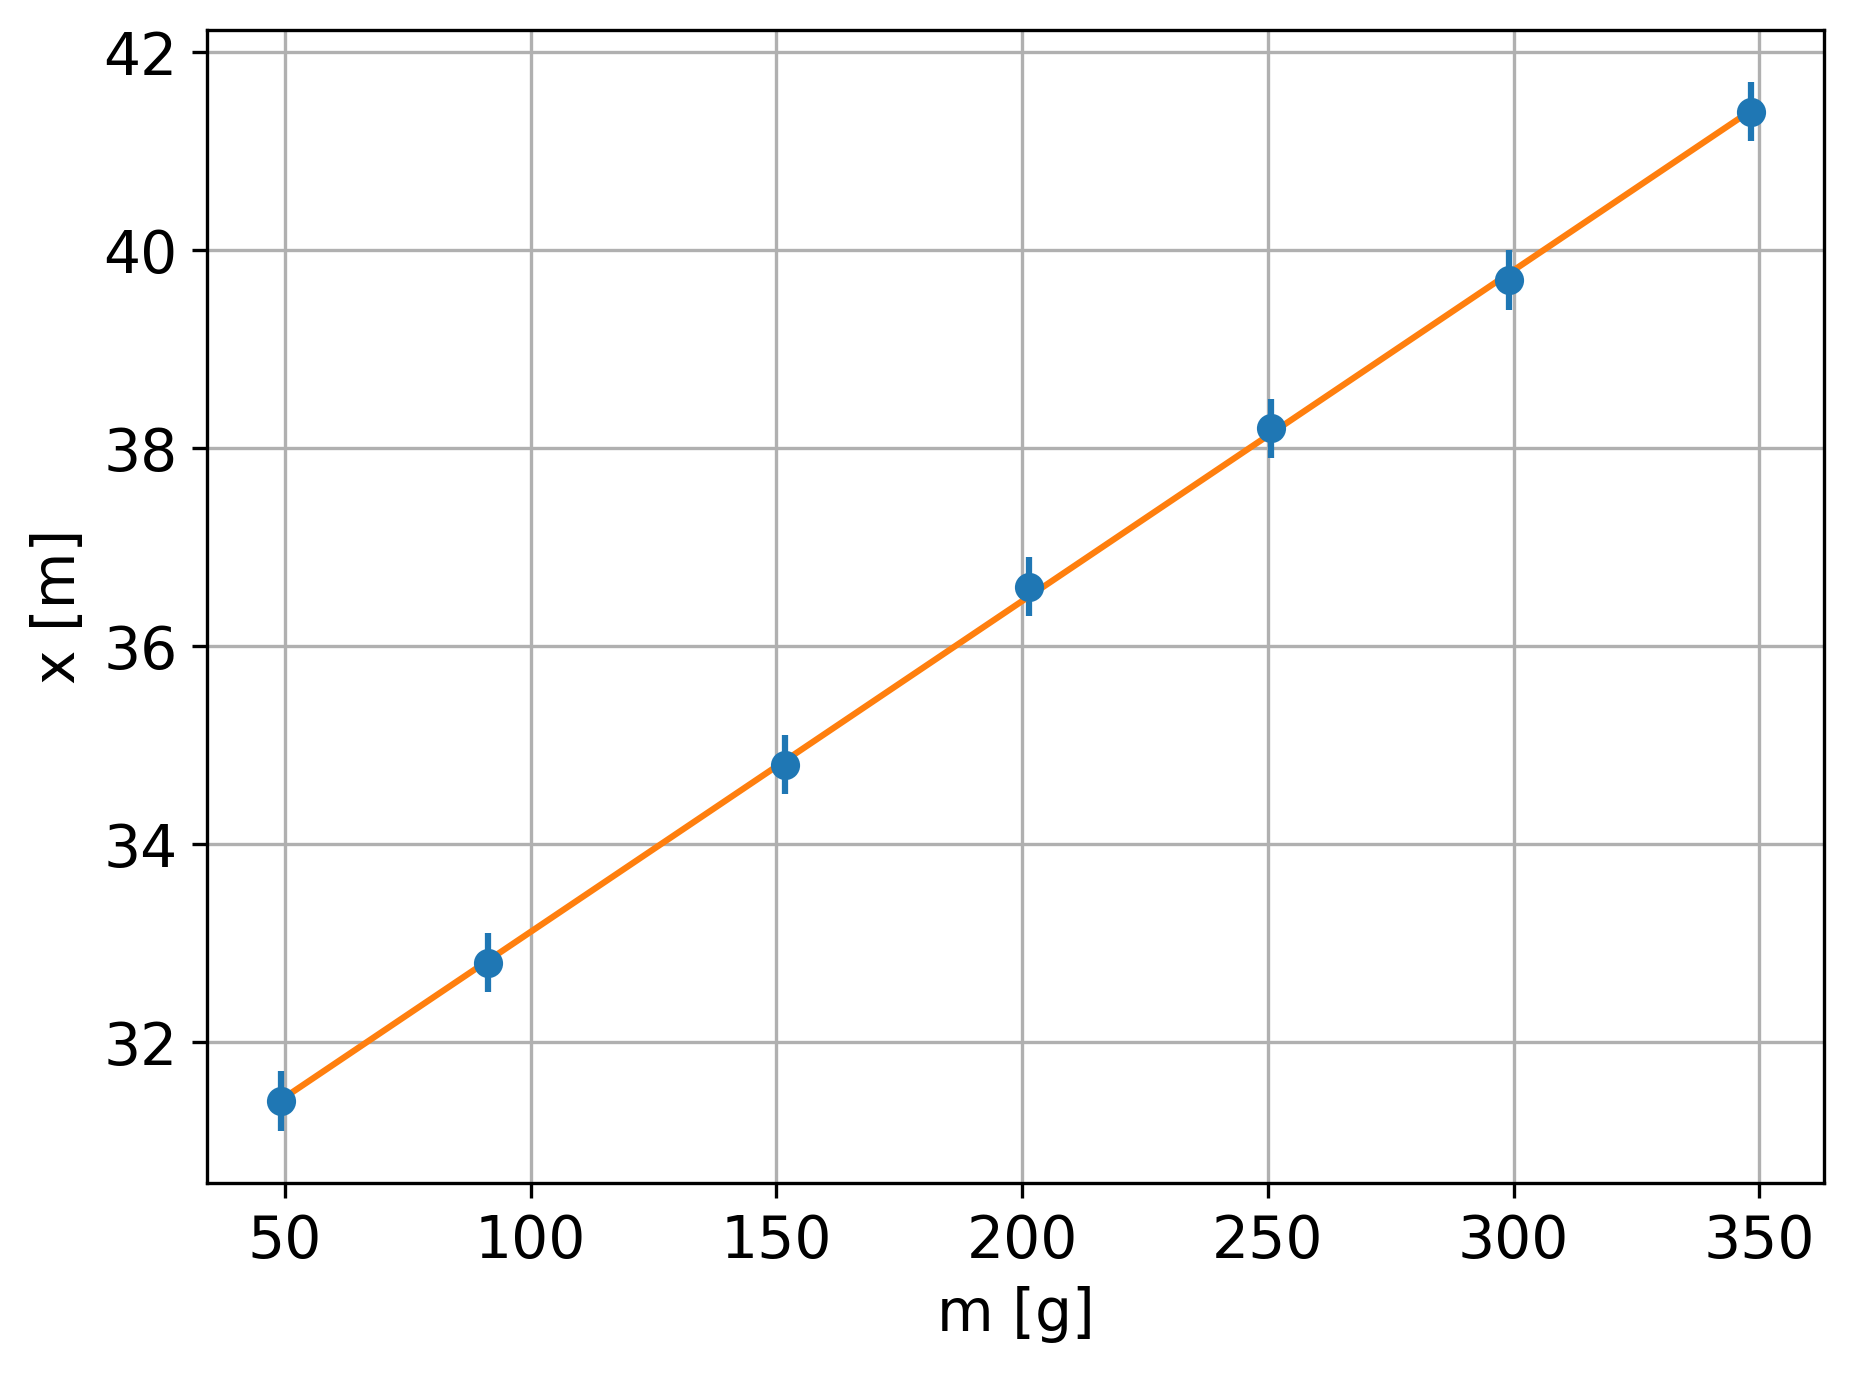
\includegraphics[scale=0.6]{spring_mass}
	\caption{Zależność długości sprężyny od zawieszonej masy wraz z dopasowaniem liniowym.}
	\label{fig:spring_mass}
\end{figure}
Wyznaczone parametry krzywej wynoszą
\[
	a = (0{,}03344 \pm 0{,}00024)\,\mathrm{cm\,g^{-1}}, \quad b = (29{,}77 \pm 0{,}06)\,\mathrm{cm}.
\]
Na podstawie parametru \(a\) obliczamy stałą sprężystości
\[
	k_0 = \frac{g}{a} = (29{,}34 \pm 0{,}21)\,\mathrm{N\,m^{-1}}.
\]

\subsection{Pomiar dynamiczny}
Za pomocą dwóch czujników PASCO PS-3219 rejestrowaliśmy położenia obu identycznych wahadeł w funkcji czasu; zebrane dane znajdują się w pliku dołączonym do dokumentu. Zawiera on trzy serie pomiarowe (po dwa pomiary): najpierw dudnienia, a następnie drgania w przeciwfazie, każdorazowo dla trzech odległości sprężyny od osi obrotu wahadła. Ostatnia seria dotyczy jednego wahadła bez podłączonej sprężyny. We wszystkich poniższych pomiarach błąd transformacji Fouriera przyjmujemy równy połowie jej rozdzielczości, \(\tfrac{f_s}{2N}\), gdzie \(f_s = 40\,\mathrm{Hz}\) oznacza częstotliwość próbkowania, a \(N\) liczbę próbek w danej serii pomiarowej. Wyznaczana tą metodą częstotliwość była praktycznie identyczna dla obu wahadeł: różnice pojawiały się poza miejscem cyfr znaczących, dlatego ignorujem tę różnicę. Kluczowa w naszych pomiarach jest odległość środka masy, wyznaczona jako \(r = (79{,}7 \pm 0{,}1) \,\mathrm{cm}\) poprzez balansowanie wachadła na cieńkiej płytce, oraz masa wahadła \(m = (3000 \pm 40)\,\mathrm{g}\). Przy pomiarach odległości od osi \(a\) zakładamy, że różnica pomiędzy wahadłami mieści się w granicach błędu pomiarowego, więc możemy ją pominąć.

\subsection{Wahadło bez sprężyny i drgania w przeciwfazie}

\begin{figure}[H]
	\centering
	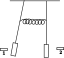
\includegraphics[scale=1]{diagram}
	\caption{Diagram układu pomiarowego stosowanego w eksperymencie. Widoczne są dwa wahadła oraz dwa czujniki odległości 1 i 2.}
	\label{fig:diagram}
\end{figure}

Analizę danych rozpoczynamy od przypadku bez podłączonej sprężyny, w którym badamy zachowanie pojedynczego wahadła.
\begin{figure}[H]
	\centering
	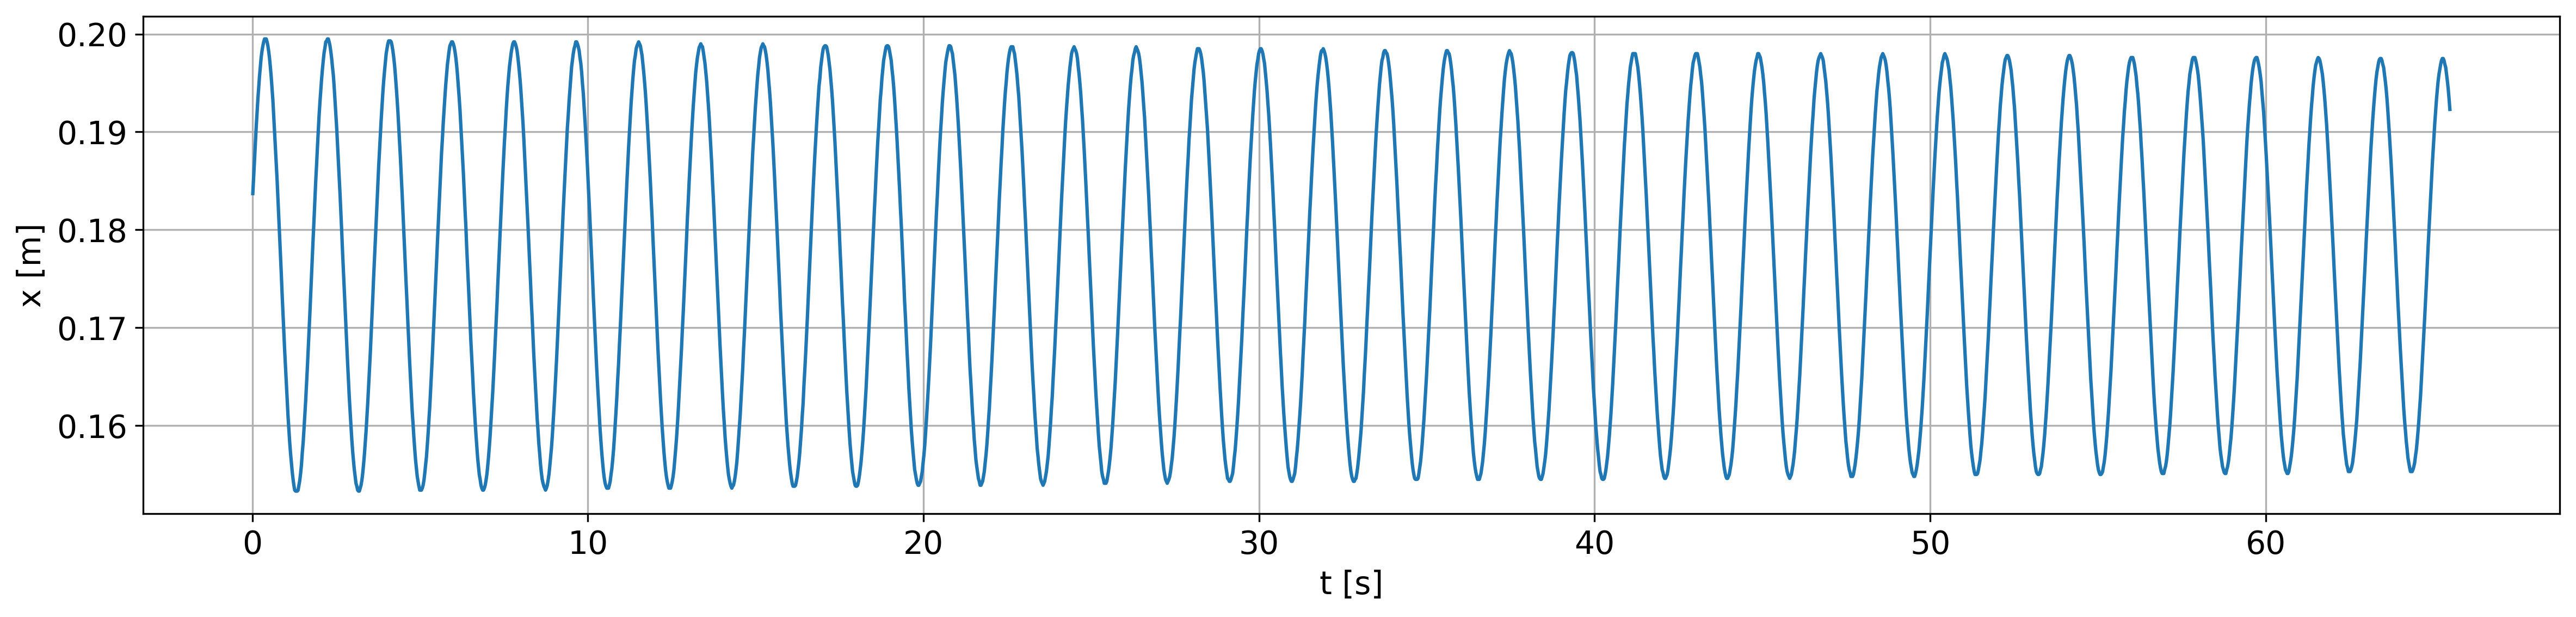
\includegraphics[width=\linewidth]{no_spring}
	\caption{Wychylenie wahadła bez sprężyny w funkcji czasu.}
	\label{fig:pendulum_nospring}
\end{figure}
\begin{figure}[H]
	\centering
	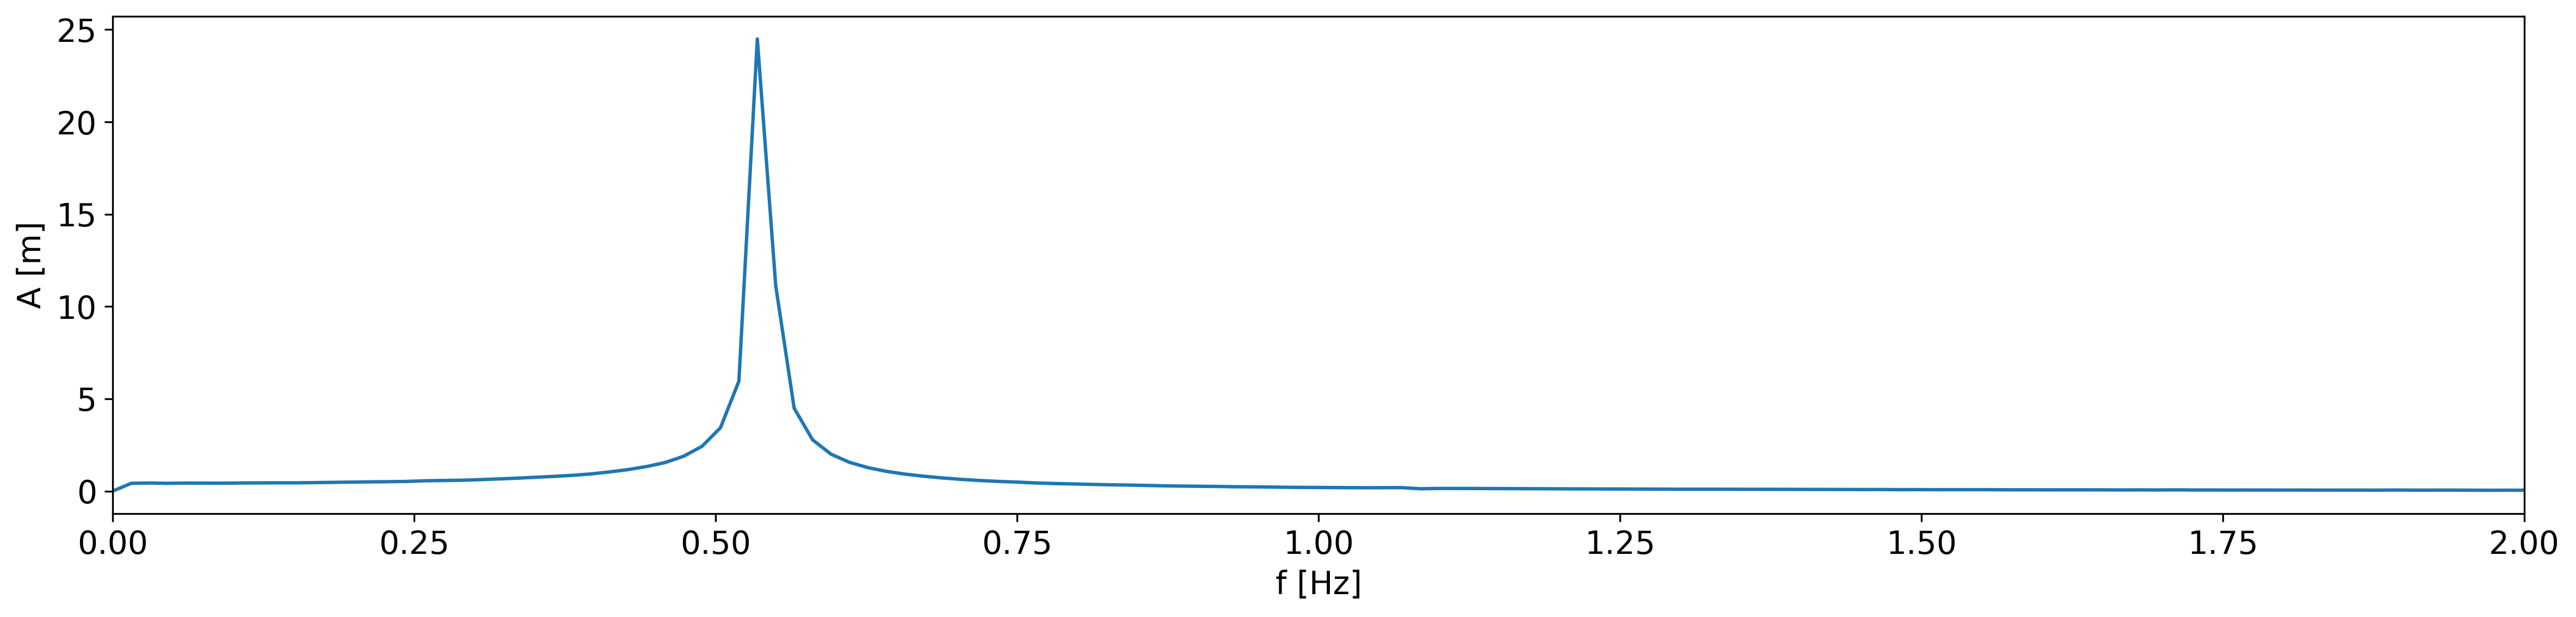
\includegraphics[width=\linewidth]{no_spring_fft}
	\caption{Transformacja Fouriera danych z rys.~\ref{fig:pendulum_nospring}.}
	\label{fig:pendulum_nospring_fft}
\end{figure}
Uzyskana częstotliwość wynosi
\[
	f_0 = (0{,}5346 \pm 0{,}008)\,\mathrm{Hz}.
\]
Wiadomo, że częstotliwość drgań wahadła spełnia\cite{skrypt}
\[
	\omega_1^2 = (2\pi f_0)^2 = \frac{mgr}{I}.
\]
Stąd moment bezwładności wynosi
\[
	I = \frac{mgr}{(2\pi f_0)^2} = (2{,}08 \pm 0{,}07)\,\mathrm{kg\,m^2}.
\]

Przeanalizujemy teraz zachowanie wahadeł drgających w przeciwfazie dla różnych punktów zaczepienia sprężyny. Częstotliwości wyznaczamy z transformacji Fouriera.

\newpage

\(d = (30 \pm 0{,}1)\,\mathrm{cm}\)
\begin{figure}[H]
	\centering
	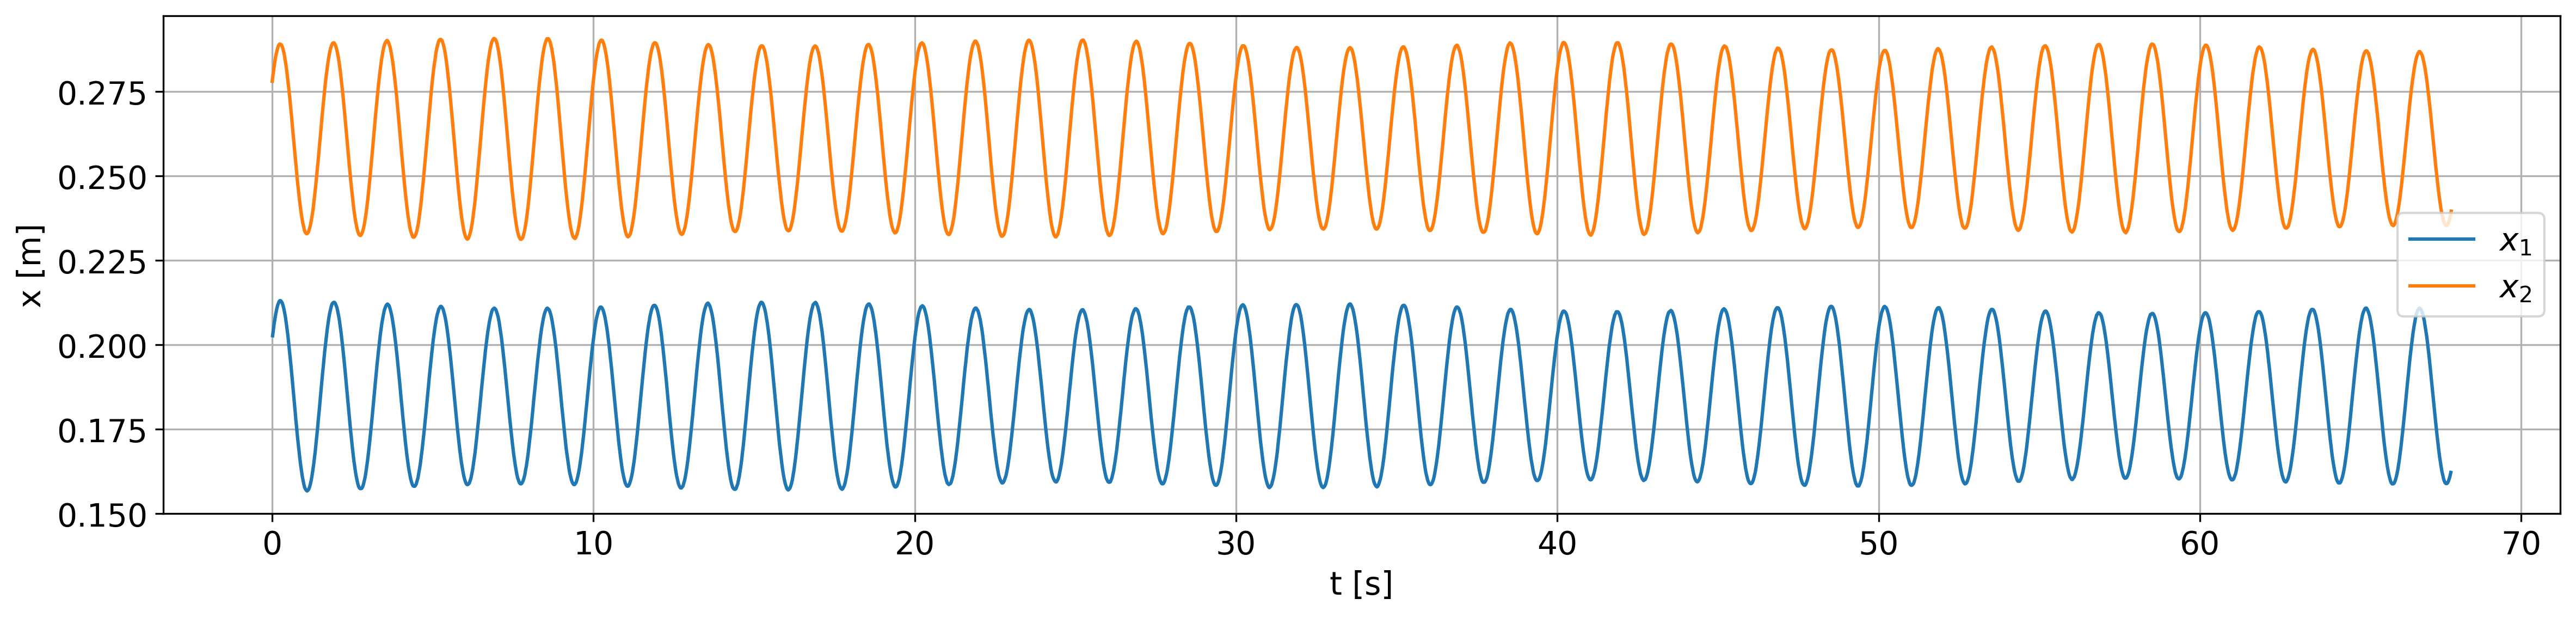
\includegraphics[width=\linewidth]{counterphase_1}
	\caption{Wychylenia lewego (\(x_1\)) i prawego (\(x_2\)) wahadła w funkcji czasu przy drganiach w przeciwfazie dla \(d = (30 \pm 0{,}1)\,\mathrm{cm}\).}
	\label{fig:counter_phase_0}
\end{figure}
\begin{figure}[H]
	\centering
	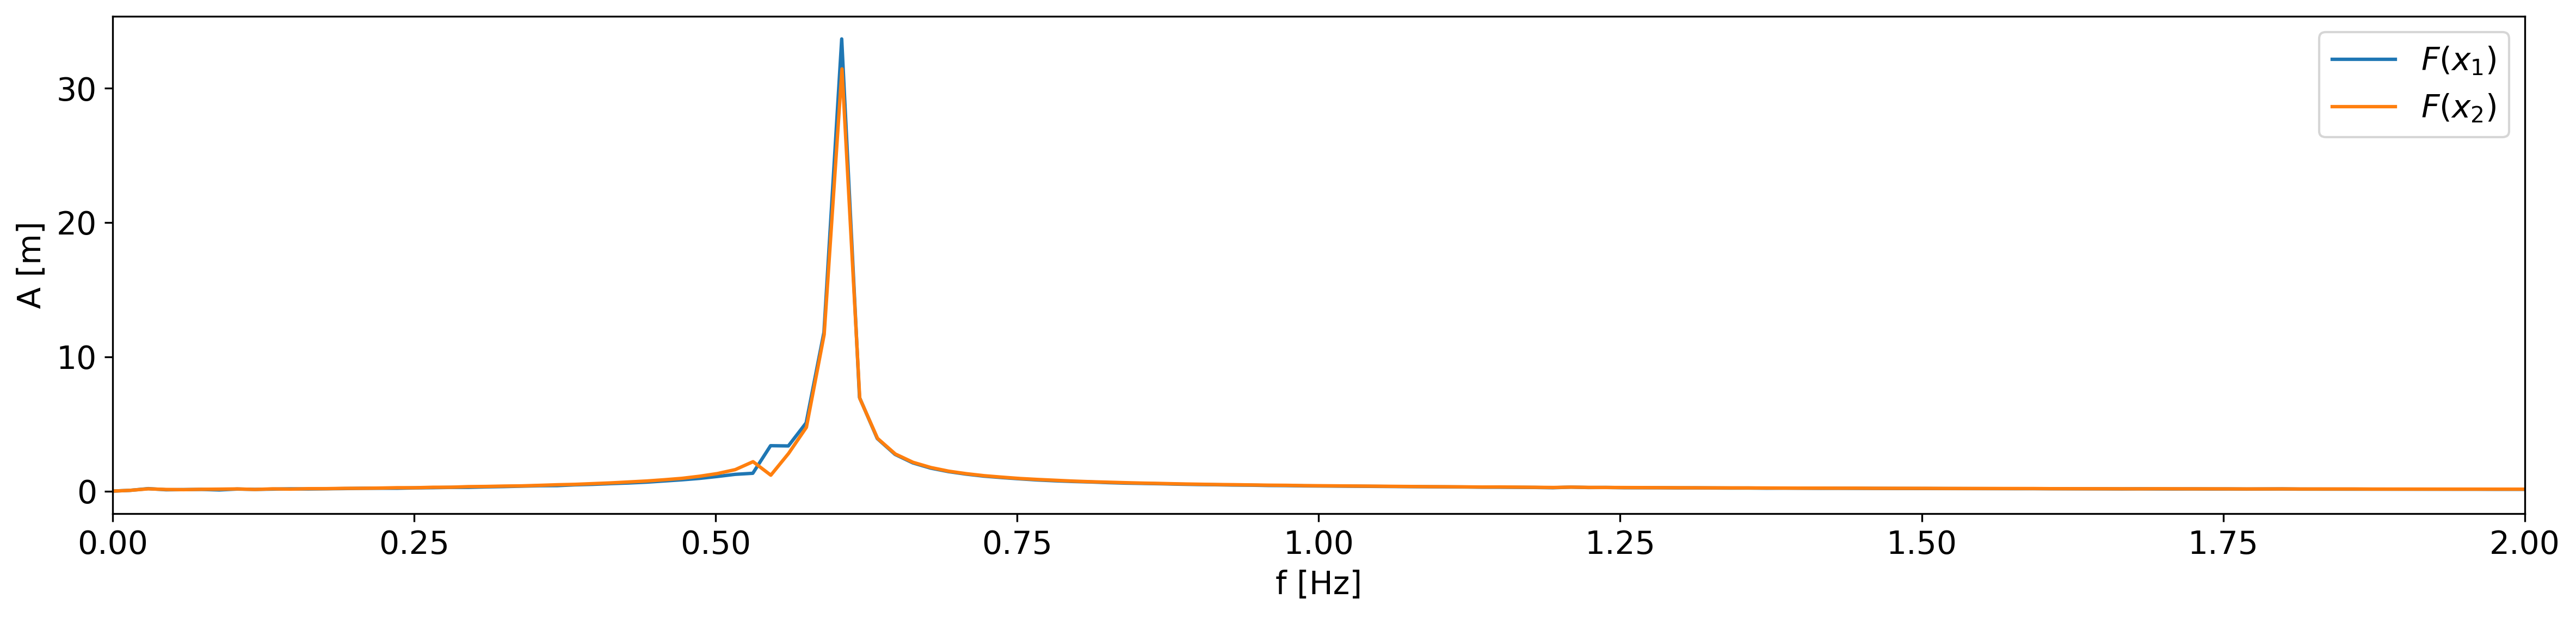
\includegraphics[width=\linewidth]{counterphase_1_fft}
	\caption{Transformacja Fouriera danych z rys.~\ref{fig:counter_phase_0}.}
	\label{fig:coutner_phase_0_fft}
\end{figure}
\[
	f_{p_1} = (0{,}6045 \pm 0{,}008)\,\mathrm{Hz}.
\]

\(d = (40 \pm 0{,}1)\,\mathrm{cm}\)
\begin{figure}[H]
	\centering
	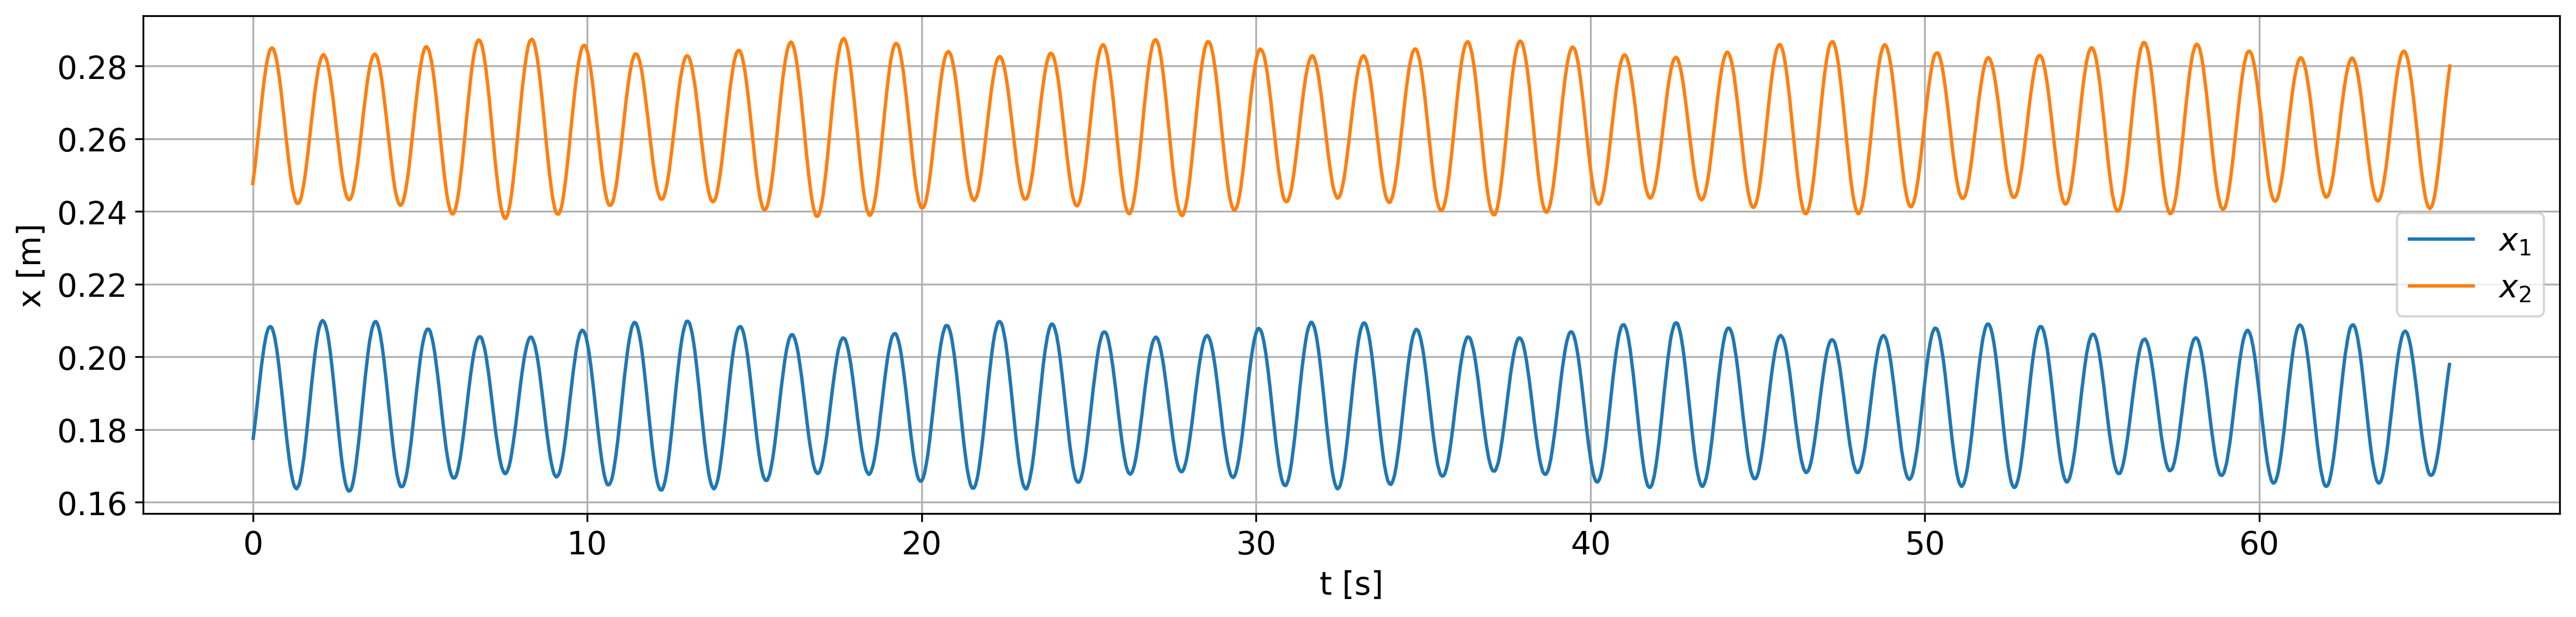
\includegraphics[width=\linewidth]{counterphase_2}
	\caption{Wychylenia lewego (\(x_1\)) i prawego (\(x_2\)) wahadła w funkcji czasu przy drganiach w przeciwfazie dla \(d = (40 \pm 0{,}1)\,\mathrm{cm}\).}
	\label{fig:counter_phase_1}
\end{figure}
\begin{figure}[H]
	\centering
	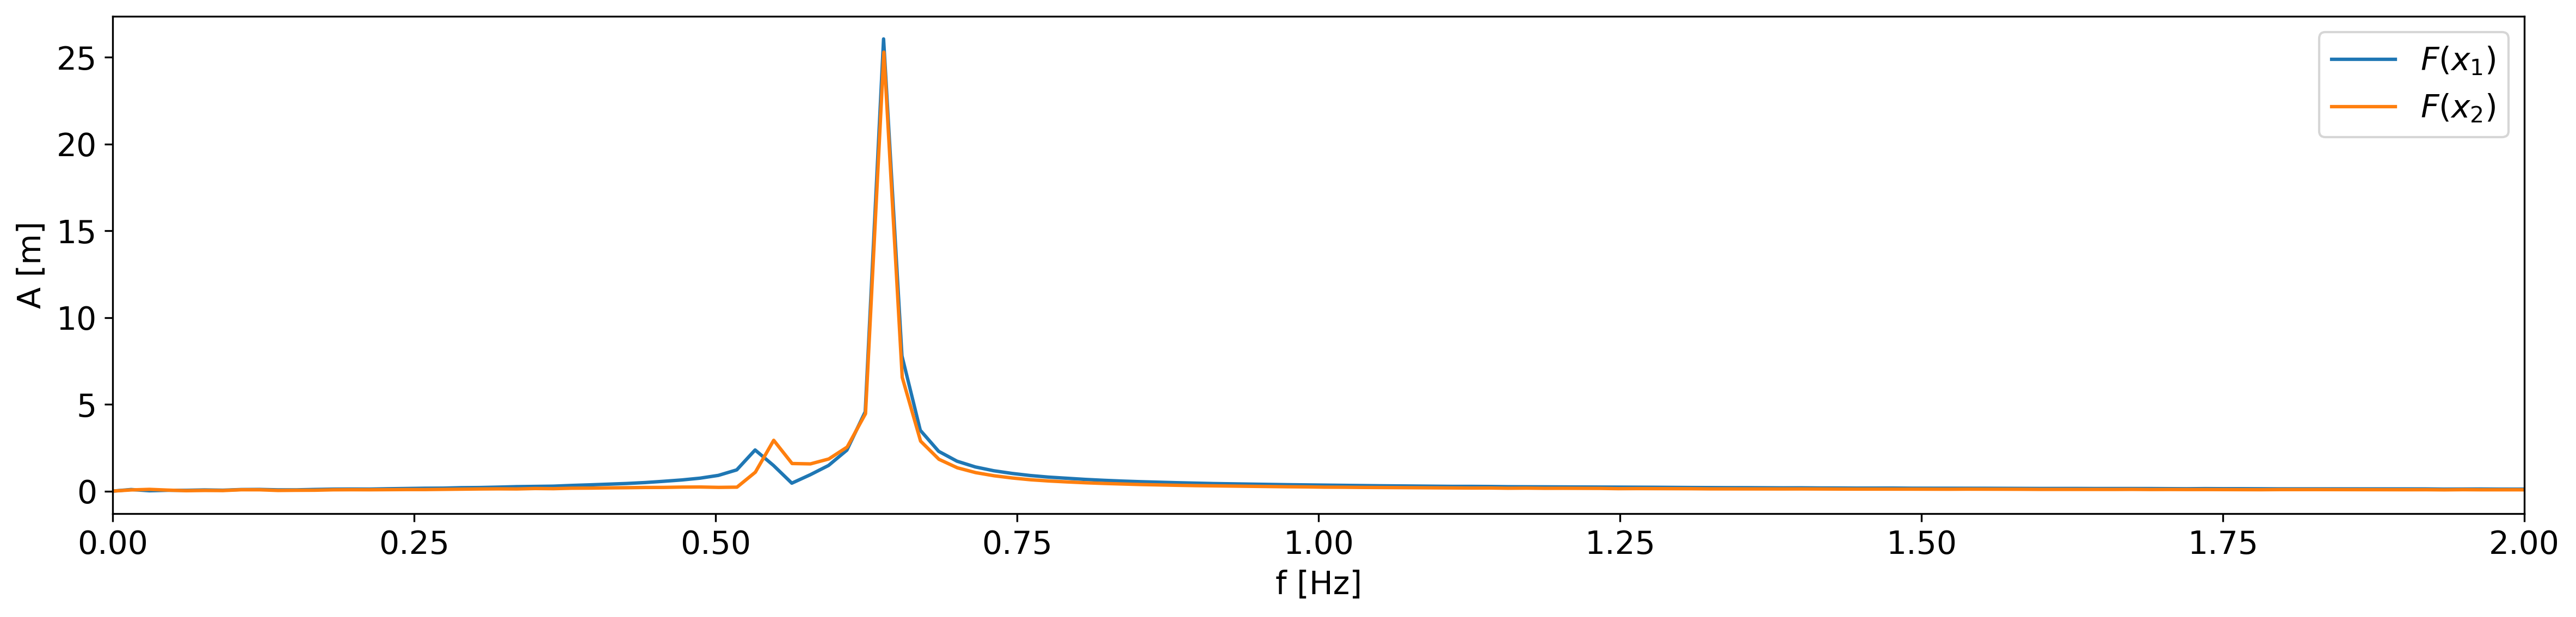
\includegraphics[width=\linewidth]{counterphase_2_fft}
	\caption{Transformacja Fouriera danych z rys.~\ref{fig:counter_phase_1}.}
	\label{fig:coutner_phase_1_fft}
\end{figure}
\[
	f_{p_2} = (0{,}639 \pm 0{,}008)\,\mathrm{Hz}.
\]

\(d = (45 \pm 0{,}1)\,\mathrm{cm}\)
\begin{figure}[H]
	\centering
	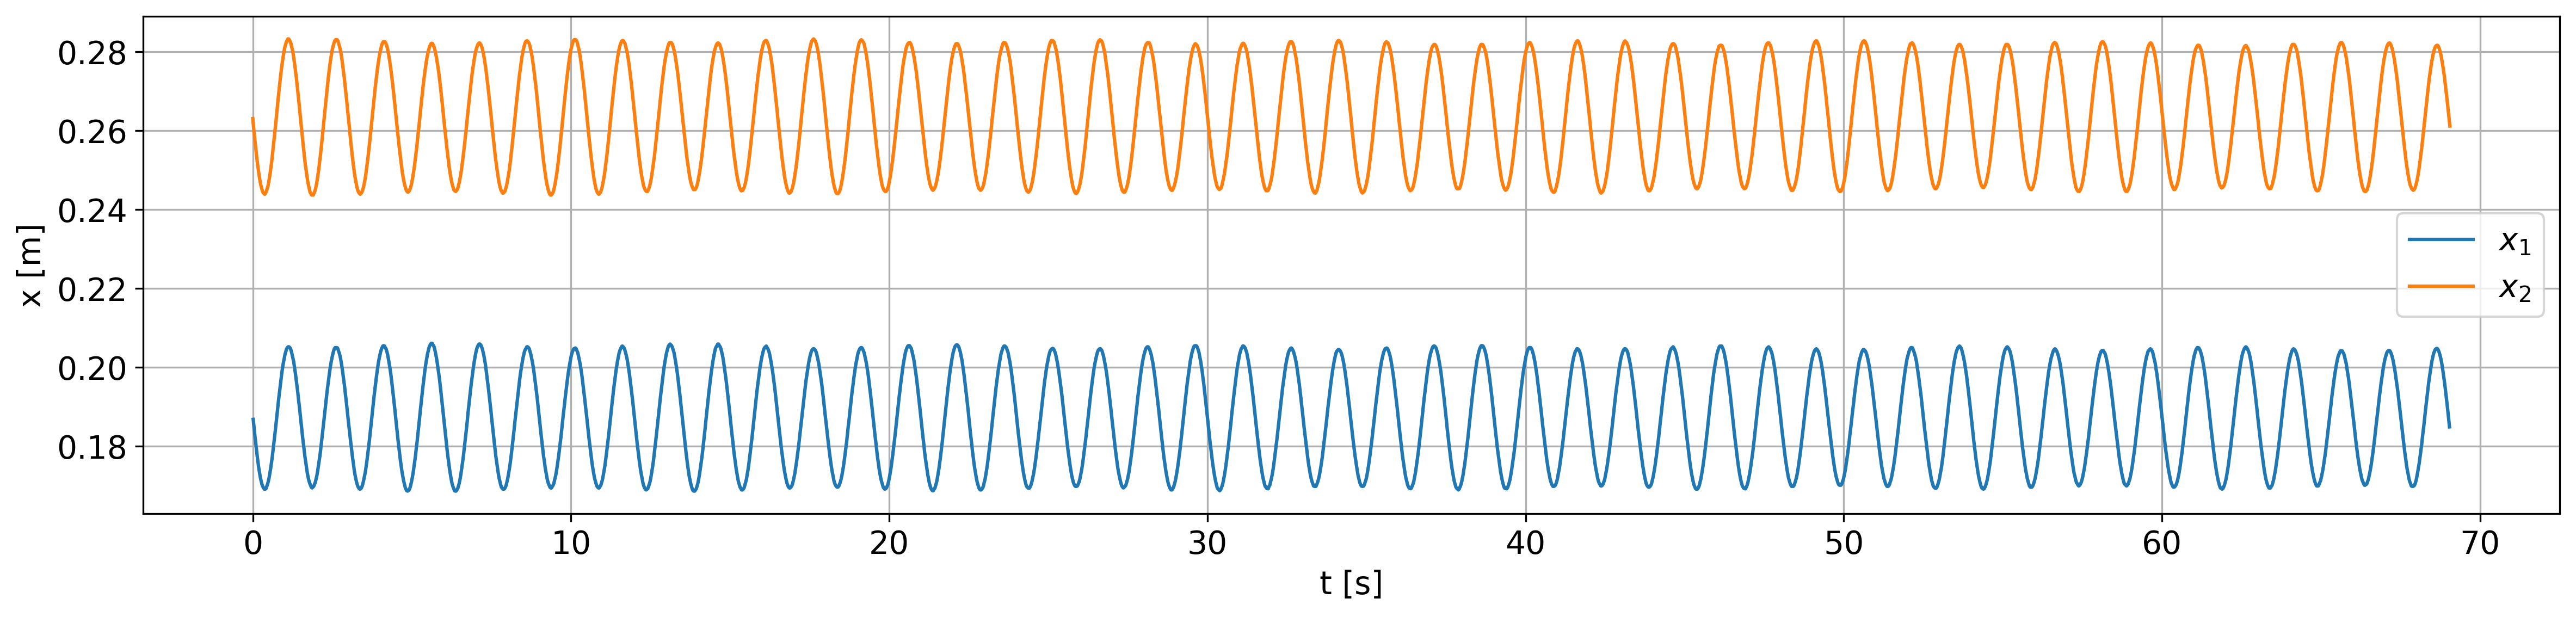
\includegraphics[width=\linewidth]{counterphase_3}
	\caption{Wychylenia lewego (\(x_1\)) i prawego (\(x_2\)) wahadła w funkcji czasu przy drganiach w przeciwfazie dla \(d = (45 \pm 0{,}1)\,\mathrm{cm}\).}
	\label{fig:counter_phase_2}
\end{figure}
\begin{figure}[H]
	\centering
	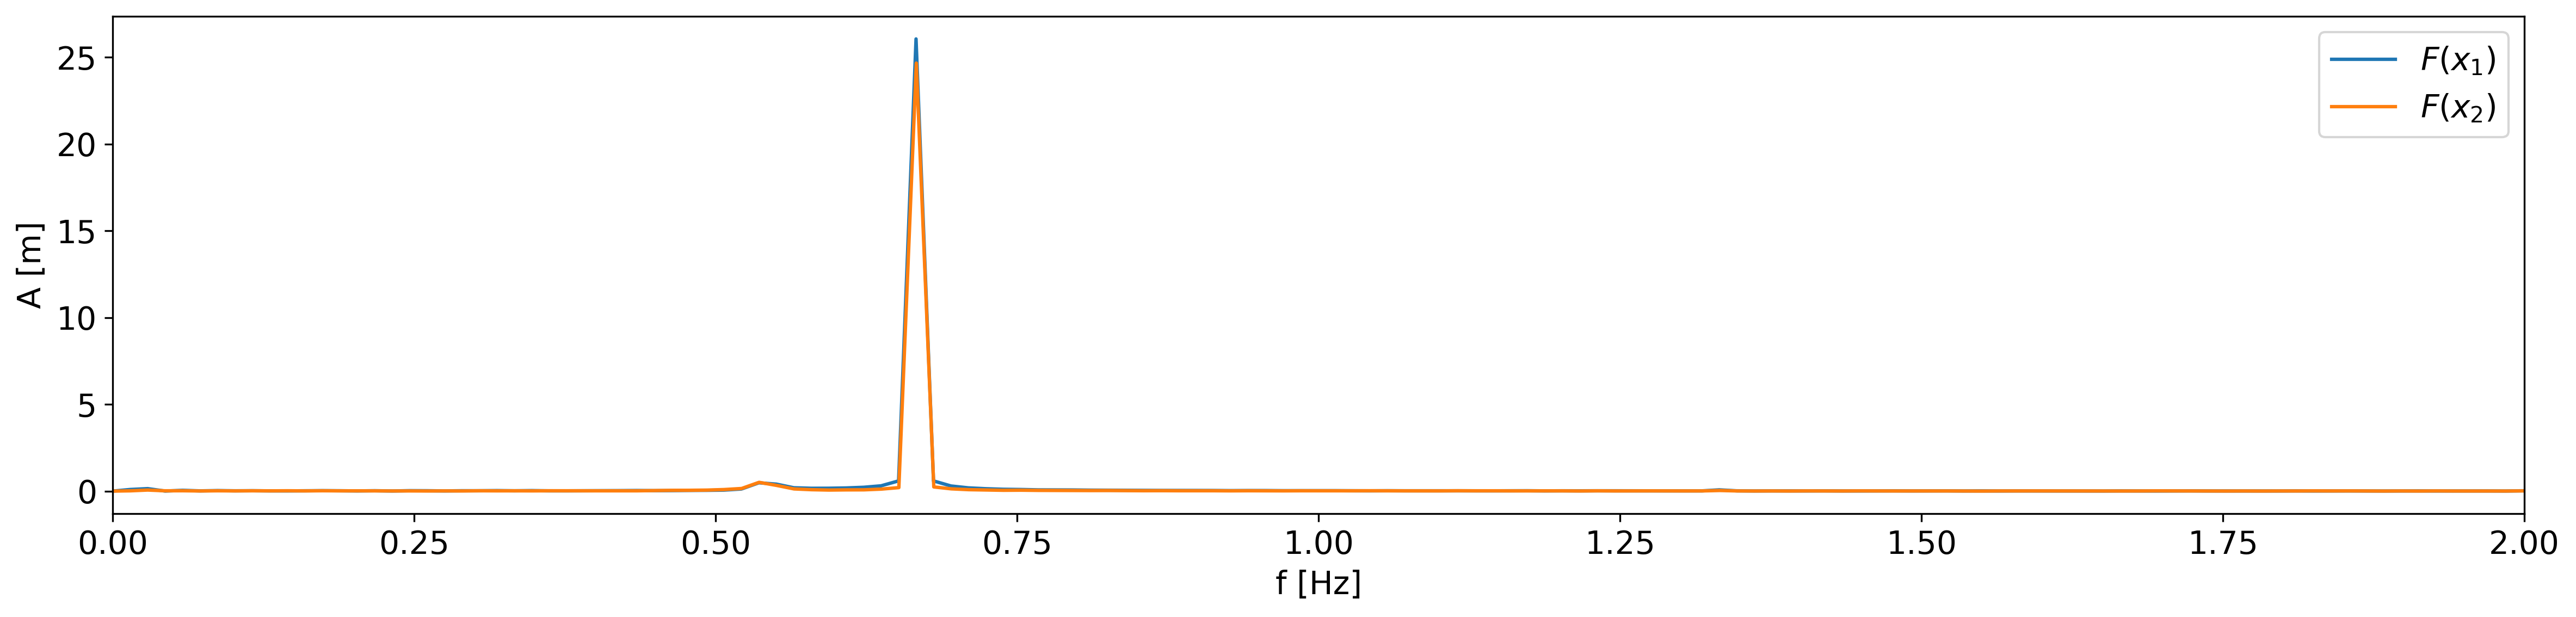
\includegraphics[width=\linewidth]{counterphase_3_fft}
	\caption{Transformacja Fouriera danych z rys.~\ref{fig:counter_phase_2}.}
	\label{fig:coutner_phase_2_fft}
\end{figure}
\[
	f_{p_3} = (0{,}666 \pm 0{,}008)\,\mathrm{Hz}.
\]

Dla przeciwfazy częstotliwość drgań spełnia\cite{skrypt}
\[
	\omega_2^2 = (2\pi f_p)^2 = \frac{mgr + 2ka^2}{I}.
\]
Wykorzystując wyniki dla drgań bez sprężyny, możemy zapisać
\[
	k = 2\pi^2 I \frac{f_p^2 - f_0^2}{a^2}.
\]
Otrzymujemy
\[
	k_1 = (36 \pm 6)\,\mathrm{N\,m^{-1}}, \quad
	k_2 = (32 \pm 4)\,\mathrm{N\,m^{-1}}, \quad
	k_3 = (32 \pm 3)\,\mathrm{N\,m^{-1}}.
\]
Średnia ważona z tych wyników wynosi
\[
	k_p = (32{,}4 \pm 2{,}0)\,\mathrm{N\,m^{-1}}.
\]

\subsection{Dudnienie}
Zbadamy teraz dudnienie wahadeł, również wyznaczając częstotliwości metodą transformacji Fouriera.

\(d = (30 \pm 0{,}1)\,\mathrm{cm}\)
\begin{figure}[H]
	\centering
	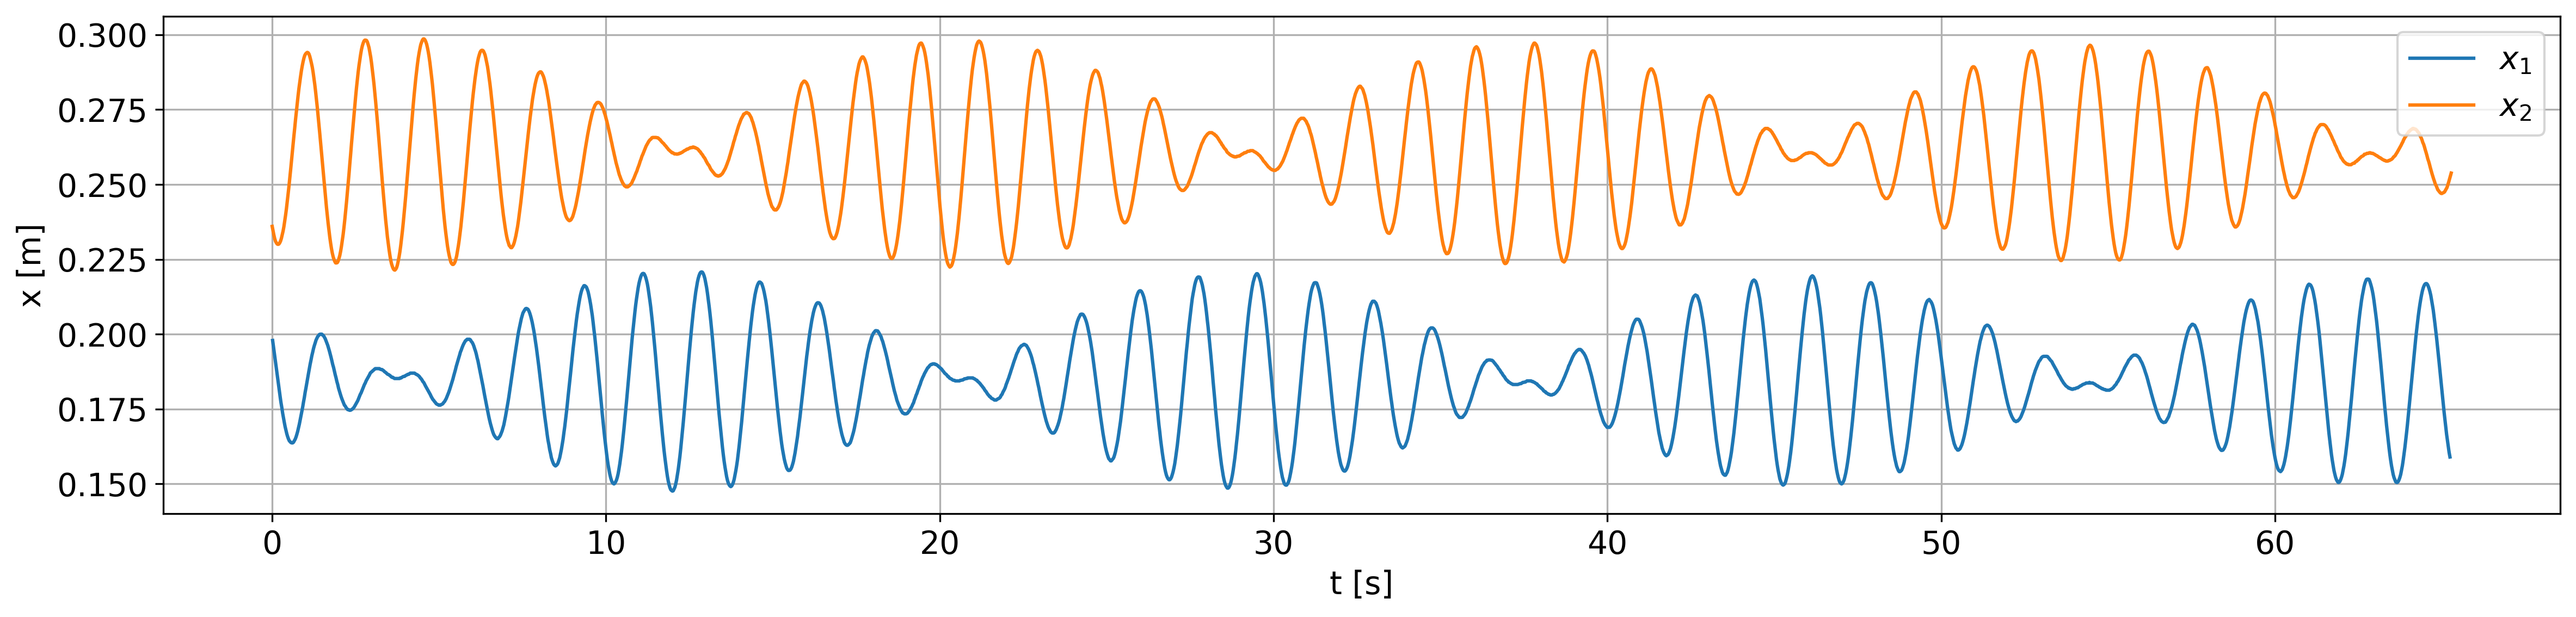
\includegraphics[width=\linewidth]{beats_1}
	\caption{Wychylenia lewego (\(x_1\)) i prawego (\(x_2\)) wahadła w funkcji czasu przy dudnieniu dla \(d = (30 \pm 0{,}1)\,\mathrm{cm}\).}
	\label{fig:beats_0}
\end{figure}
\begin{figure}[H]
	\centering
	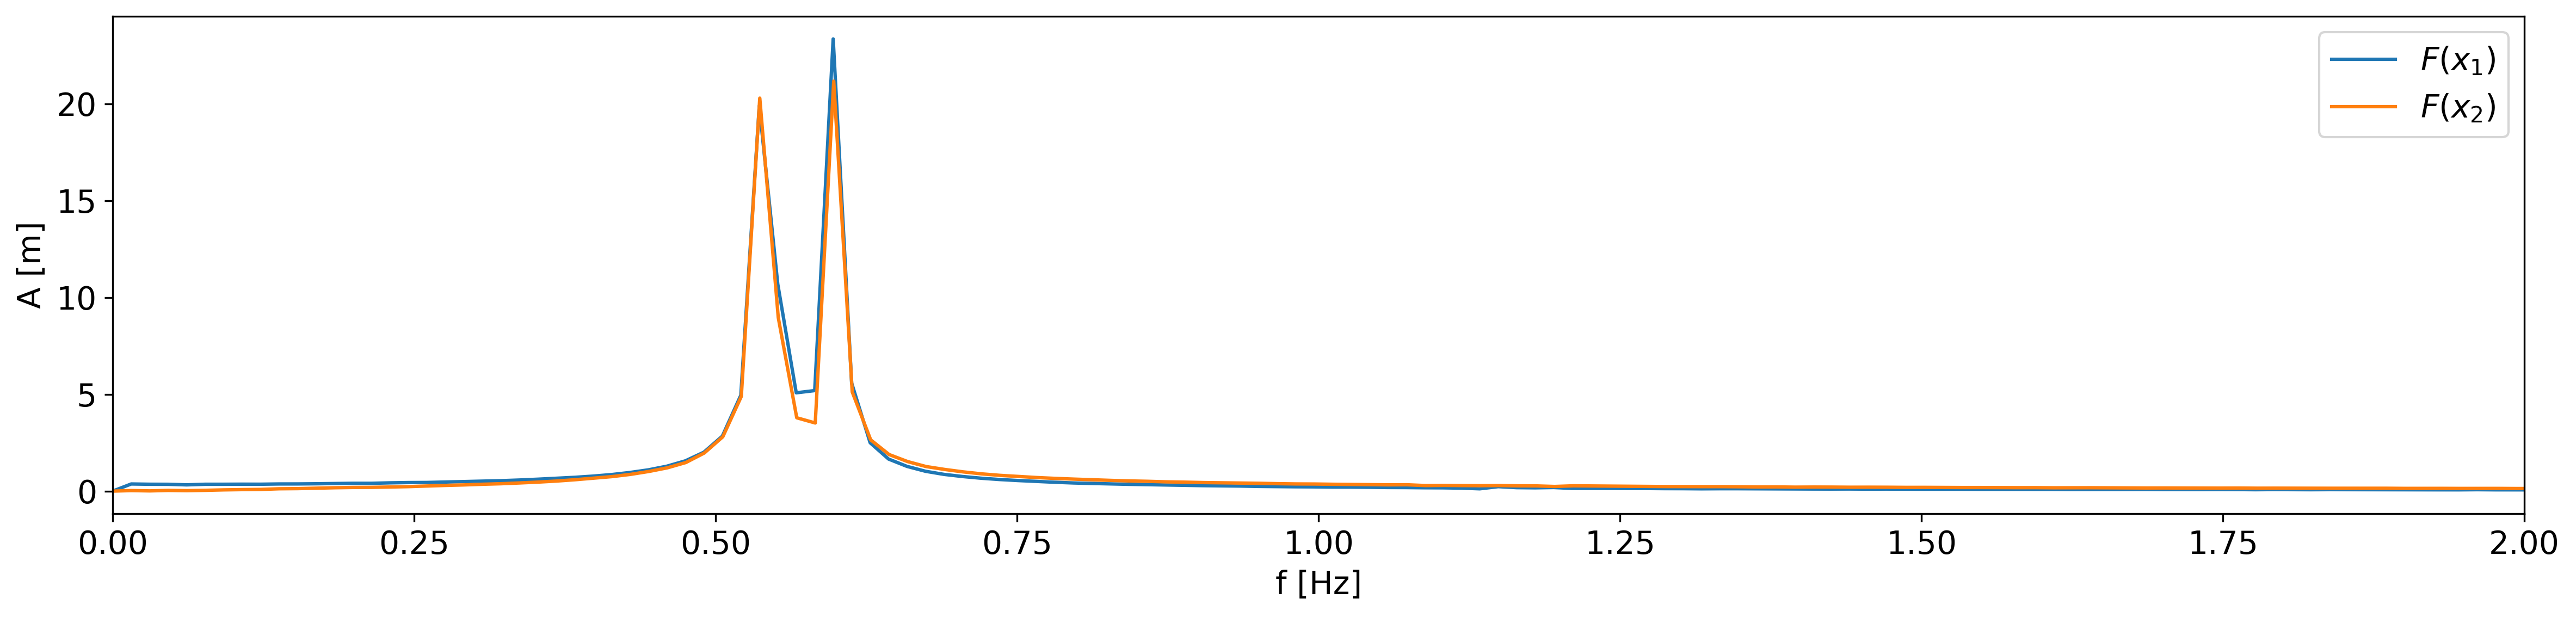
\includegraphics[width=\linewidth]{beats_1_fft}
	\caption{Transformacja Fouriera danych z rys.~\ref{fig:beats_0}.}
	\label{fig:coutner_phase_0_fft}
\end{figure}
\[
	f_{d_{10}} = (0{,}536 \pm 0{,}016)\,\mathrm{Hz}, \quad
	f_{d_{11}} = (0{,}598 \pm 0{,}008)\,\mathrm{Hz}.
\]

\newpage

\(d = (40 \pm 0{,}1)\,\mathrm{cm}\)
\begin{figure}[H]
	\centering
	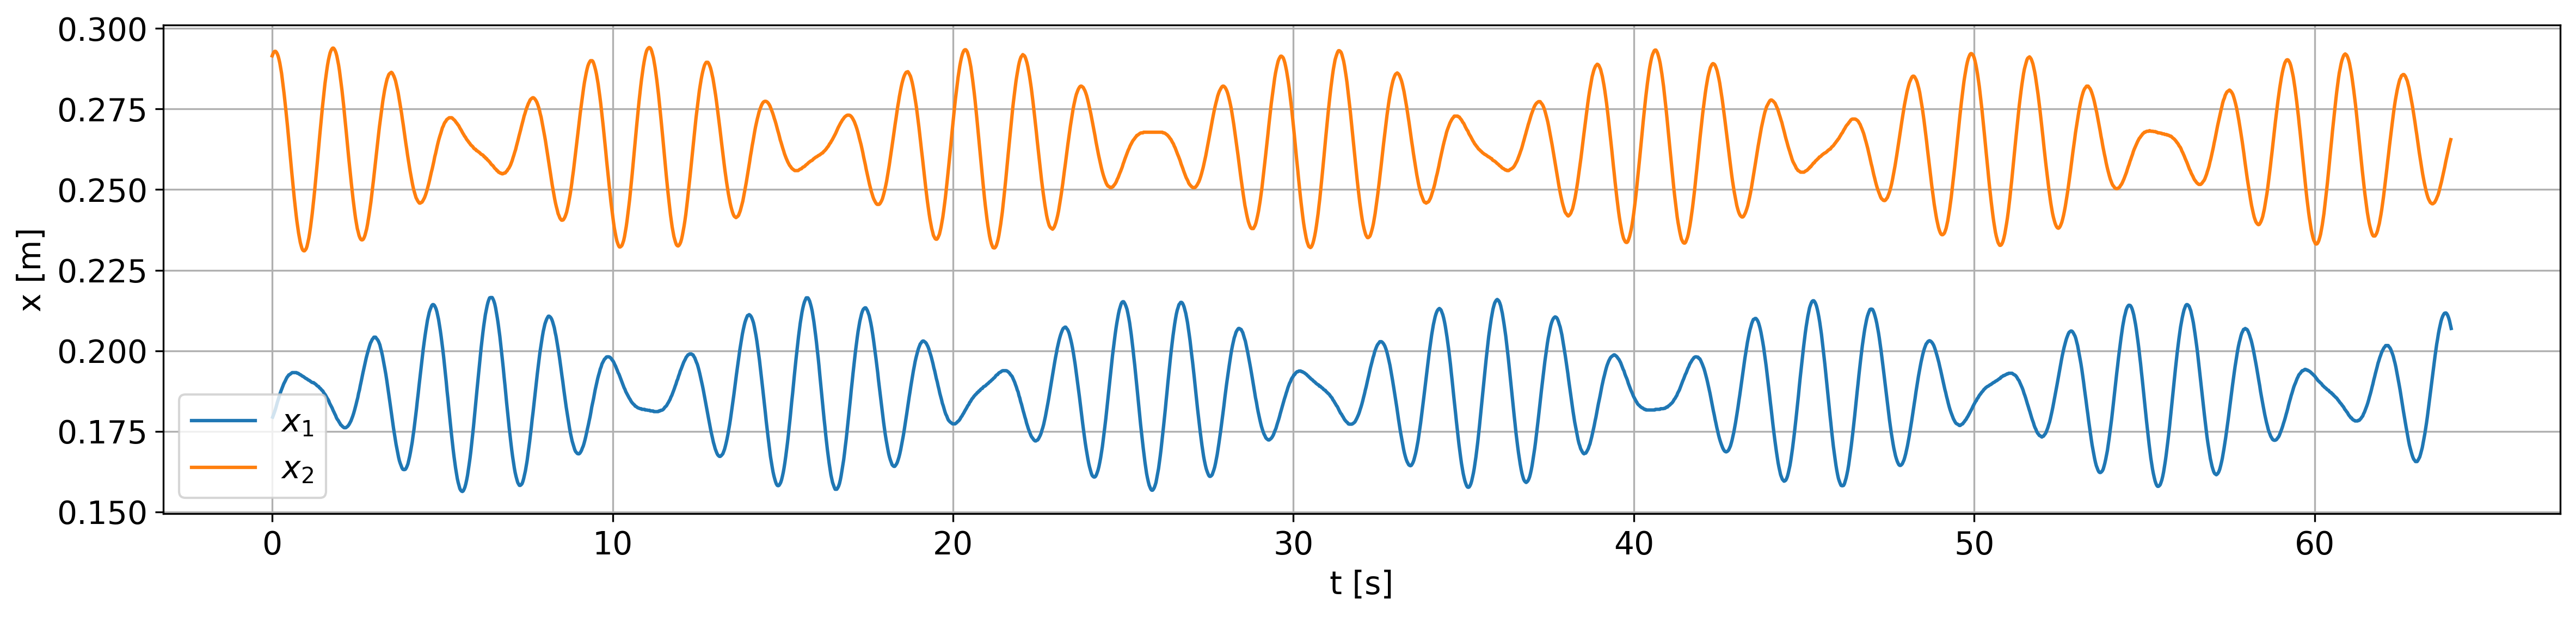
\includegraphics[width=\linewidth]{beats_2}
	\caption{Wychylenia lewego (\(x_1\)) i prawego (\(x_2\)) wahadła w funkcji czasu przy dudnieniu dla \(d = (40 \pm 0{,}1)\,\mathrm{cm}\).}
	\label{fig:beats_1}
\end{figure}
\begin{figure}[H]
	\centering
	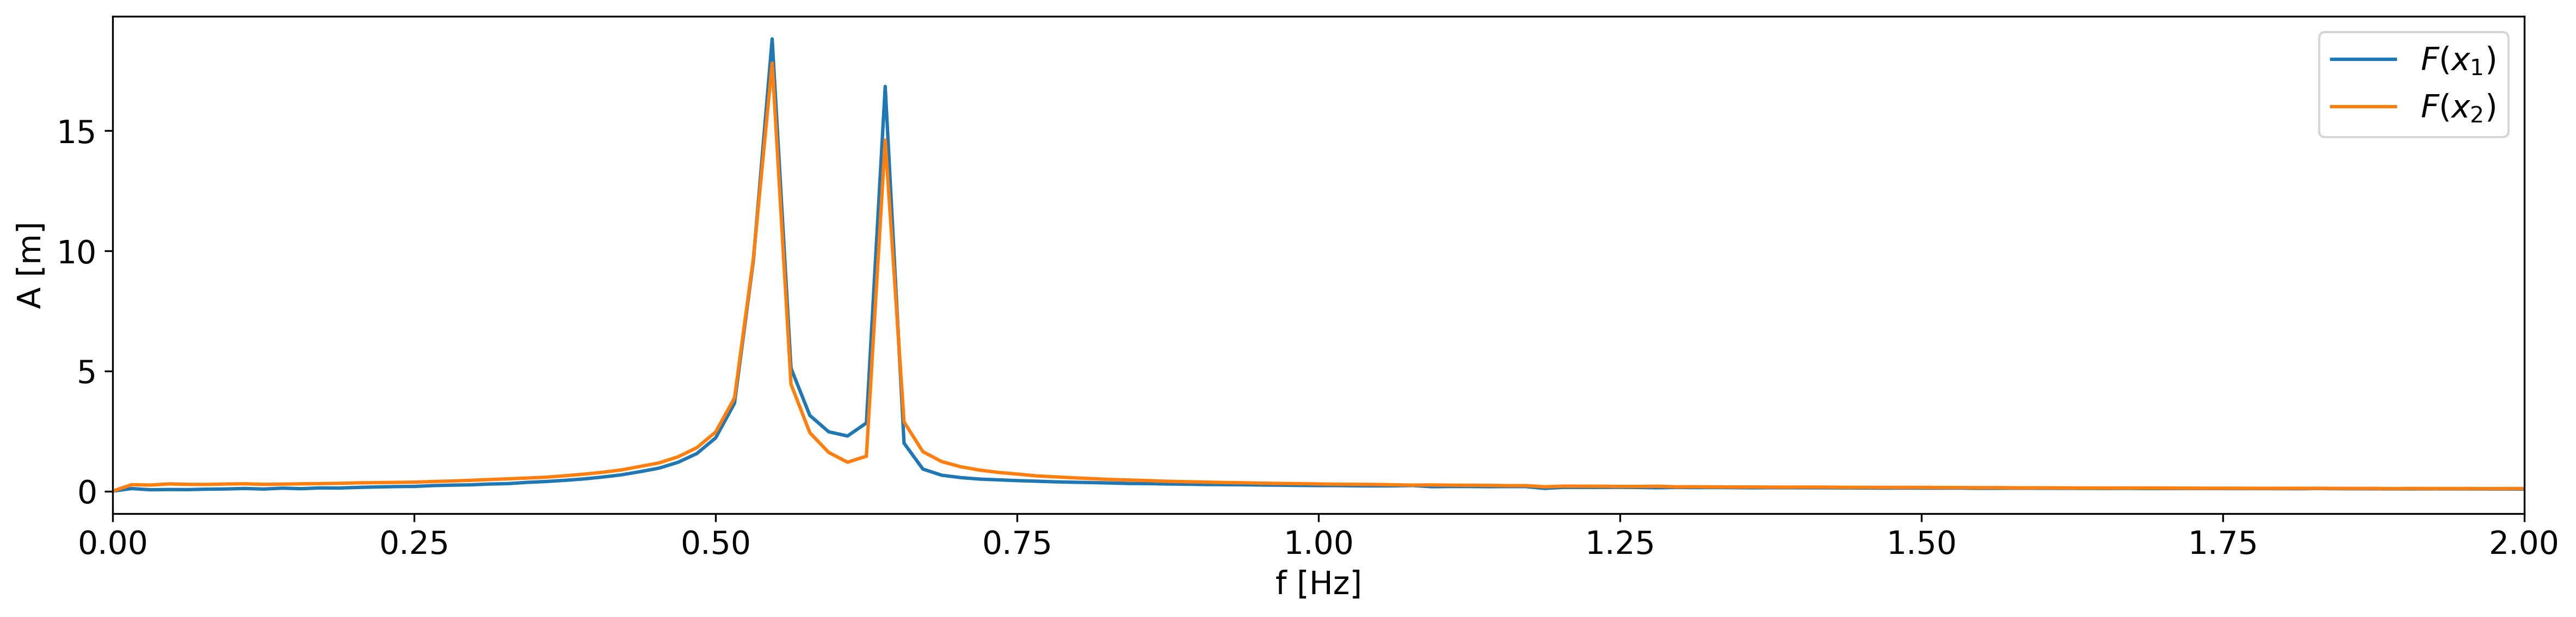
\includegraphics[width=\linewidth]{beats_2_fft}
	\caption{Transformacja Fouriera danych z rys.~\ref{fig:beats_1}.}
	\label{fig:coutner_phase_1_fft}
\end{figure}
\[
	f_{d_{20}} = (0{,}547 \pm 0{,}016)\,\mathrm{Hz}, \quad
	f_{d_{21}} = (0{,}641 \pm 0{,}008)\,\mathrm{Hz}.
\]

\(d = (45 \pm 0{,}1)\,\mathrm{cm}\)
\begin{figure}[H]
	\centering
	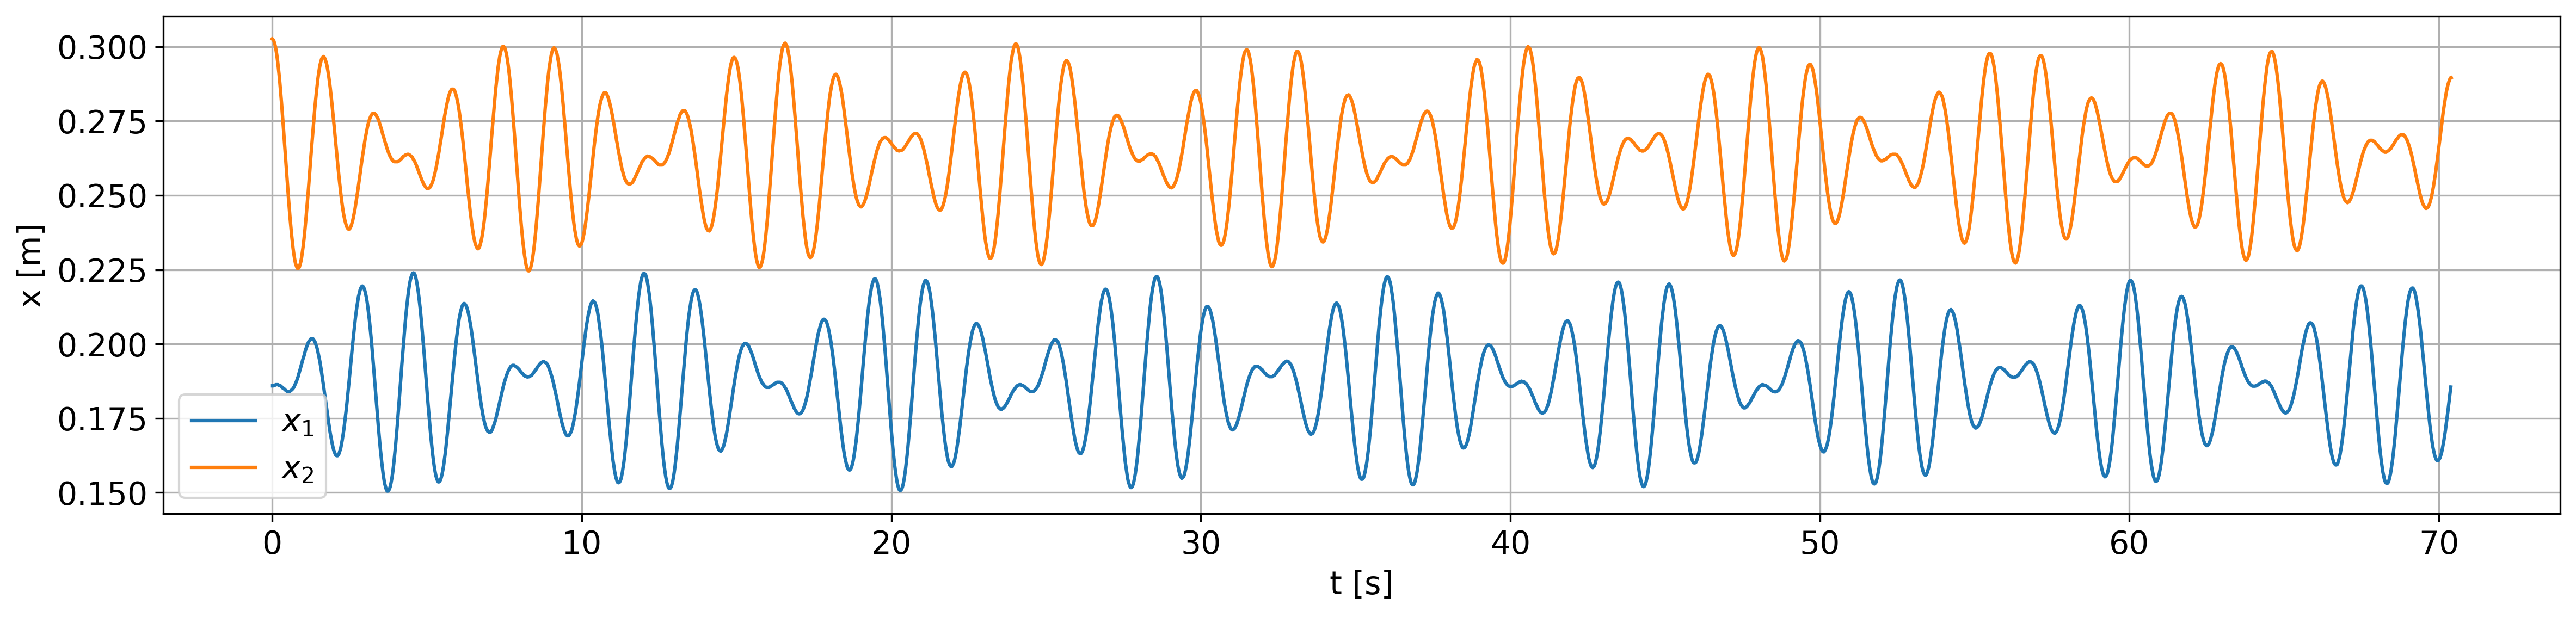
\includegraphics[width=\linewidth]{beats_3}
	\caption{Wychylenia lewego (\(x_1\)) i prawego (\(x_2\)) wahadła w funkcji czasu przy dudnieniu dla \(d = (45 \pm 0{,}1)\,\mathrm{cm}\).}
	\label{fig:beats_2}
\end{figure}
\begin{figure}[H]
	\centering
	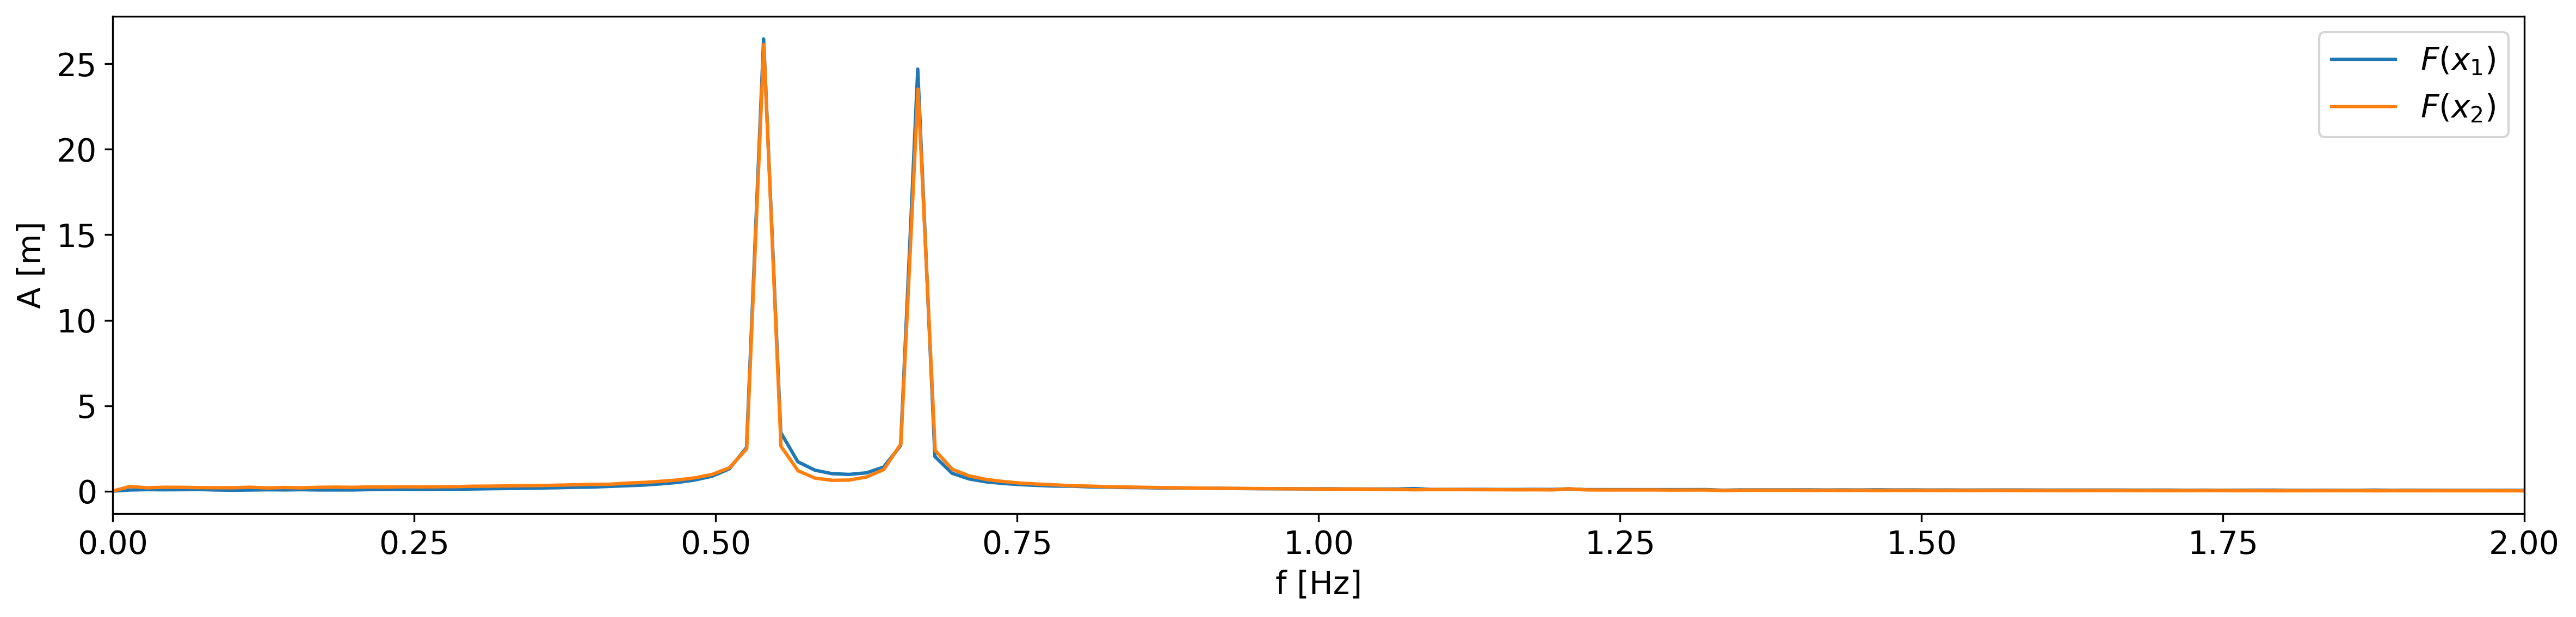
\includegraphics[width=\linewidth]{beats_3_fft}
	\caption{Transformacja Fouriera danych z rys.~\ref{fig:beats_2}.}
	\label{fig:coutner_phase_2_fft}
\end{figure}
\[
	f_{d_{30}} = (0{,}540 \pm 0{,}055)\,\mathrm{Hz}, \quad
	f_{d_{31}} = (0{,}668 \pm 0{,}007)\,\mathrm{Hz}.
\]

Dwie częstotliwości występujące podczas dudnienia odpowiadają częstotliwościom własnym układu\cite{skrypt}, dlatego możemy powtórzyć analizę z poprzedniego przypadku, korzystając z wzorów
\[
	I = \frac{mgr}{(2\pi f_{d0})^2}, \qquad
	k = 2\pi^2 I \frac{f_{d1}^2 - f_{d0}^2}{a^2}.
\]
Otrzymujemy
\[
	I_1 = (2{,}07 \pm 0{,}07)\,\mathrm{kg\,m^2}, \quad
	I_2 = (1{,}99 \pm 0{,}07)\,\mathrm{kg\,m^2}, \quad
	I_3 = (2{,}04 \pm 0{,}07)\,\mathrm{kg\,m^2},
\]
\[
	k_1 = (32 \pm 6)\,\mathrm{N\,m^{-1}}, \quad
	k_2 = (27 \pm 4)\,\mathrm{N\,m^{-1}}, \quad
	k_3 = (31 \pm 3)\,\mathrm{N\,m^{-1}}.
\]
Z tych wyników wyznaczamy średnią ważoną
\[
	k_d = (29{,}6 \pm 2{,}0)\,\mathrm{N\,m^{-1}}.
\]

\section{Podsumowanie}
Z otrzymanych wyników wynika, że najdokładniejszą metodą okazało się wyznaczanie stałej sprężystości poprzez statyczne podwieszanie ciężarków, które dało rezultat \(k_0 = (29{,}34 \pm 0{,}21)\,\mathrm{N\,m^{-1}}\). Obie metody wykorzystujące wahadła charakteryzują się tym samym błędem, jednak analiza dudnień dostarczyła wyniku bliższego wartości statycznej, \(k_d = (29{,}6 \pm 2{,}0)\,\mathrm{N\,m^{-1}}\), podczas gdy badanie fazy i przeciwfazy oddzielnie zaowocowało \(k_p = (32{,}4 \pm 2{,}0)\,\mathrm{N\,m^{-1}}\). Błąd w metodzie statycznej wynika głównie z trudności w dokładnym określeniu długości sprężyny, której nie można dotykać, aby nie zaburzyć długości oraz drobnych drgań sprężyny. Dla pomiarów z wahadłami największe znaczenie ma niepewność wynikająca z transformacji Fouriera; jej zmniejszenie wymagałoby dłuższych rejestracji. Warto zauważyć, że błąd był mniejszy dla większych wartości \(a\), które zwiększały wpływ sprężyny w pomiarach. Z kolei analiza dudnień jest dokładniejsza od sztucznego rozdzielania drgań własnych, ponieważ w jej trakcie nie występuje przerwa czasowa, w której układ mógłby ulec nieznacznym zmianom wpływającym na wynik końcowy.

\newpage

\begin{thebibliography}{1}

	\bibitem{skrypt}
	\emph{Wahadła sprzężone}, Aneta Drabińska, Roman J. Nowak i Andrzej Witowski, Uniwersytet Warszawski.

\end{thebibliography}

\end{document}
